\section{Lecture 14: More on QAOA: Cost and Mixer Hamiltonians, Full
Circuit}\label{sec:lecture14}

\subsubsection*{Review}

\qs{QAOA Components}{
  What are the two main components that alternate in a QAOA circuit?
}

\sol{
  The two main components are:
  \begin{enumerate}
    \item \textbf{Cost evolution operator}: $e^{-i\gamma_p H_C}$, which
      encodes the problem's objective function

    \item \textbf{Mixing evolution operator}: $e^{-i\beta_p H_M}$, which
      explores the solution space
  \end{enumerate}
}

%%%%%%%%%%%%

\vspace{0.3cm}

\index{Quantum Approximate Optimization Algorithms!Cost Hamiltonians}
\subsubsection*{Cost Hamiltonians in Detail}

\dfn{Cost Hamiltonian}{The \textbf{Cost Hamiltonian} $H_C$ in QAOA encodes
  the objective function of the optimization problem. It is designed such that
  its ground state (lowest energy eigenstate) corresponds to the optimal
solution of the classical problem.}

\vspace{0.3cm}

\noindent
\textbf{Properties of Cost Hamiltonians:}
\begin{itemize}
  \item \textbf{Diagonal in computational basis}: $H_C$ is typically diagonal
    in the $Z$-basis, making measurements straightforward.

  \item \textbf{Problem-specific}: Each optimization problem requires a
    different $H_C$.

  \item \textbf{Locality}: Many practical $H_C$ terms involve only a few
    qubits (e.g., 2-local terms like $Z_i Z_j$ for \textsc{Max-Cut}).
\end{itemize}


\noindent
\ex{Max-$k$-SAT Cost Hamiltonian}{
  For the Max-$k$-SAT problem, each clause $c$ is encoded as an operator
  $C_c$. For example, the clause $(x_1 \lor \lnot x_2 \lor x_3)$ is encoded as:
  \[
    C_c = \frac{I - Z_1}{2} \cdot \frac{I + Z_2}{2} \cdot \frac{I - Z_3}{2}
  \]

  The overall cost Hamiltonian is:
  \[
    H_C = \sum_{c} \frac{1-C_c}{2}
  \]

  This gives higher energy to states that satisfy more clauses.
}

\begin{figure}[H]
  \centering
  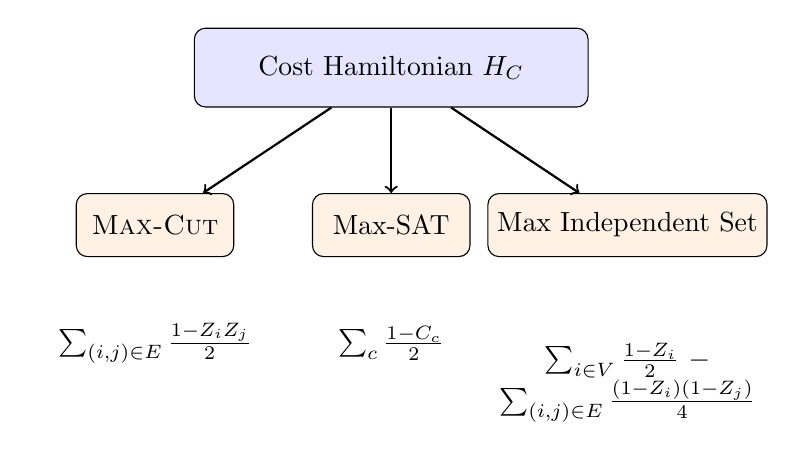
\begin{tikzpicture}
    \node[draw, rounded corners, fill=blue!10, minimum width=5cm, minimum height=1cm] (cost) at (0,0) {Cost Hamiltonian $H_C$};

    \node[draw, rounded corners, fill=orange!10, minimum width=2cm, minimum height=0.8cm] (maxcut) at (-3,-2) {\textsc{Max-Cut}};
    \node[draw, rounded corners, fill=orange!10, minimum width=2cm, minimum height=0.8cm] (maxsat) at (0,-2) {Max-SAT};
    \node[draw, rounded corners, fill=orange!10, minimum width=3.5cm, minimum height=0.8cm] (mis) at (3,-2) {Max Independent Set};

    \draw[->, thick] (cost) -- (maxcut);
    \draw[->, thick] (cost) -- (maxsat);
    \draw[->, thick] (cost) -- (mis);

    \node[align=center, text width=3cm] at (-3,-3.5) {$\sum_{(i,j) \in E} \frac{1-Z_i Z_j}{2}$};
    \node[align=center, text width=3cm] at (0,-3.5) {$\sum_{c} \frac{1-C_c}{2}$};
    \node[align=center, text width=3.5cm] at (3,-4) {$\sum_{i \in V} \frac{1-Z_i}{2} - \sum_{(i,j) \in E} \frac{(1-Z_i)(1-Z_j)}{4}$};
  \end{tikzpicture}
  \caption{Different cost Hamiltonians for various optimization problems}
  \label{fig:cost-hamiltonians}
\end{figure}

\vspace{0.3cm}

\index{Quantum Approximate Optimization Algorithms!Implementing Cost Hamiltonians}
\subsubsection*{Implementing Cost Hamiltonians}

The operator $e^{-i\gamma H_C}$ can be challenging to implement directly.
When $H_C$ consists of terms that commute with each other, we can decompose
the exponential:

\[
  e^{-i\gamma H_C} = e^{-i\gamma \sum_j h_j} = \prod_j e^{-i\gamma h_j}
\]

For the \textsc{Max-Cut} problem, each term is of the form $Z_i Z_j$, and we
can implement $e^{-i\gamma Z_i Z_j}$ using the following circuit:

\begin{figure}[H]
  \centering
  \begin{quantikz}
    \lstick{$q_i$} & \ctrl{1} & \qw & \ctrl{1} & \qw \\
    \lstick{$q_j$} & \targ{} & \gate{R_Z(2\gamma)} & \targ{} & \qw
  \end{quantikz}
  \caption{Circuit for implementing $e^{-i\gamma Z_i Z_j}$}
  \label{fig:zz-gate-implementation}
\end{figure}

\nt{
  The decomposition $e^{-i\gamma H_C} = \prod_j e^{-i\gamma h_j}$ is only
  valid when all terms $h_j$ commute. For non-commuting terms, more
  sophisticated techniques like Trotter-Suzuki decomposition are required.
}

\vspace{0.3cm}

\index{Quantum Approximate Optimization Algorithms!Mixer Hamiltonians}
\subsubsection*{Mixer Hamiltonians in Detail}

\dfn{Mixer Hamiltonian}{The \textbf{Mixer Hamiltonian} $H_M$ in QAOA drives
  the exploration of the solution space. It is typically chosen to be
  non-commuting with the cost Hamiltonian $H_C$ to enable transitions between
different states in the computational basis.}

\vspace{0.3cm}

\noindent
\textbf{Standard Mixer:}
\begin{itemize}
  \item The most common mixer is the transverse field: $H_M = \sum_{i=1}^n X_i$
  \item Implemented directly as $R_X(2\beta)$ gates on each qubit
  \item Allows exploration of the entire $2^n$ solution space
\end{itemize}

\begin{figure}[H]
  \centering
  \begin{quantikz}
    \lstick{$q_1$} & \gate{R_X(2\beta)} & \qw \\
    \lstick{$q_2$} & \gate{R_X(2\beta)} & \qw \\
    \lstick{$\vdots$} & \vdots & \vdots \\
    \lstick{$q_n$} & \gate{R_X(2\beta)} & \qw
  \end{quantikz}
  \caption{Circuit for implementing the standard mixer $e^{-i\beta \sum_i X_i}$}
  \label{fig:standard-mixer}
\end{figure}

\vspace{0.3cm}

\noindent
\textbf{Advanced Mixers:}
\begin{itemize}
  \item \textbf{Problem-specific mixers}: Designed to preserve constraints of
    the problem

  \item \textbf{XY mixers}: $H_M = \sum_{(i,j) \in E} (X_i X_j + Y_i Y_j)$
    for problems with hard constraints

  \item \textbf{Controlled mixers}: Conditionally apply mixing operations
    based on constraint satisfaction

\end{itemize}

\ex{XY Mixer for Number-Preserving Problems}{
  For problems where the total number of 1s must remain constant (e.g., graph
  coloring with a fixed number of colors), an XY mixer can be used:
  \begin{align}
    H_M^{XY} = \sum_{i < j} (X_i X_j + Y_i Y_j) = \sum_{i < j} (|01\rangle\langle10| + |10\rangle\langle01|)
  \end{align}

  This mixer only swaps 0s and 1s between qubits, preserving the total
  Hamming weight of the state. Implementation requires more complex gate
  sequences.

  \begin{figure}[H]
    \centering
    \begin{quantikz}
      \lstick{$q_i$} & \gate{H} & \ctrl{1} & \qw & \ctrl{1} & \gate{H} & \qw \\
      \lstick{$q_j$} & \gate{H} & \targ{} & \gate{R_Z(2\beta)} & \targ{} & \gate{H} & \qw
    \end{quantikz}
    \caption{Implementation of one term in the XY mixer}
    \label{fig:xy-mixer}
  \end{figure}
}

\vspace{0.3cm}

\index{Quantum Approximate Optimization Algorithms!Full QAOA Circuit}
\subsubsection*{Full QAOA Circuit Implementation}

\dfn{QAOA Circuit Depth}{The \textbf{QAOA circuit depth parameter} $P$
  determines how many alternating layers of cost and mixer operators are
  applied. Higher $P$ typically leads to better approximation quality but
increases circuit complexity.}

\vspace{0.3cm}

\noindent
\textbf{Circuit for QAOA with Depth $P$:}

\begin{figure}[H]
  \centering
  \begin{quantikz}
    \lstick{$q_1$} & \gate{H} & \gate[3]{e^{-i\gamma_1 H_C}} & \gate{R_X(2\beta_1)} & \gate[3]{e^{-i\gamma_2 H_C}} & \gate{R_X(2\beta_2)} & \ldots & \gate[3]{e^{-i\gamma_P H_C}} & \gate{R_X(2\beta_P)} & \meter{} \\
    \lstick{$q_2$} & \gate{H} & \qw & \gate{R_X(2\beta_1)} & \qw & \gate{R_X(2\beta_2)} & \ldots & \qw & \gate{R_X(2\beta_P)} & \meter{} \\
    \lstick{$q_n$} & \gate{H} & \qw & \gate{R_X(2\beta_1)} & \qw & \gate{R_X(2\beta_2)} & \ldots & \qw & \gate{R_X(2\beta_P)} & \meter{} \\
  \end{quantikz}
  \caption{General structure of a QAOA circuit with depth $P$}
  \label{fig:qaoa-general-circuit}
\end{figure}

\noindent
The circuit consists of:
\begin{enumerate}
  \item Initial state preparation: $H^{\otimes n}|0\rangle^{\otimes n}$

  \item $P$ repetitions of:
    \begin{itemize}
      \item Cost operator: $e^{-i\gamma_p H_C}$

      \item Mixer operator: $e^{-i\beta_p H_M}$
    \end{itemize}
  \item Final measurement in the computational basis

\end{enumerate}

\vspace{0.3cm}

\ex{Full \textsc{Max-Cut} QAOA Circuit for $P=2$}{
  For a 4-node cycle graph (\textsc{Max-Cut} problem) with $P=2$:

  \begin{figure}[H]
    \centering
    \begin{quantikz}
      \lstick{$q_0$} & \gate{H} & \gate{e^{-i\gamma_1 Z_0 Z_1}} & \gate{e^{-i\gamma_1 Z_0 Z_3}} & \gate{R_X(2\beta_1)} & \gate{e^{-i\gamma_2 Z_0 Z_1}} & \gate{e^{-i\gamma_2 Z_0 Z_3}} & \gate{R_X(2\beta_2)} & \meter{} \\
      \lstick{$q_1$} & \gate{H} & \qw & \gate{e^{-i\gamma_1 Z_1 Z_2}} & \gate{R_X(2\beta_1)} & \qw & \gate{e^{-i\gamma_2 Z_1 Z_2}} & \gate{R_X(2\beta_2)} & \meter{} \\
      \lstick{$q_2$} & \gate{H} & \qw & \qw & \gate{R_X(2\beta_1)} & \qw & \qw & \gate{R_X(2\beta_2)} & \meter{} \\
      \lstick{$q_3$} & \gate{H} & \qw & \gate{e^{-i\gamma_1 Z_2 Z_3}} & \gate{R_X(2\beta_1)} & \qw & \gate{e^{-i\gamma_2 Z_2 Z_3}} & \gate{R_X(2\beta_2)} & \meter{} \\
    \end{quantikz}
    \caption{QAOA circuit for \textsc{Max-Cut} on a 4-node cycle with $P=2$}
    \label{fig:maxcut-p2-circuit}
  \end{figure}

  Note that for clarity, the implementation of $e^{-i\gamma Z_i Z_j}$ with
  CNOT and $R_Z$ gates is not shown explicitly in this diagram.
}

\vspace{0.3cm}

\index{Quantum Approximate Optimization Algorithms!Parameter Optimization}
\subsubsection*{Parameter Optimization Strategies}

\dfn{QAOA Parameter Optimization}{The process of finding optimal values for
  the parameters $\gamma = (\gamma_1, \ldots, \gamma_P)$ and $\beta = (\beta_1,
  \ldots, \beta_P)$ to minimize the expectation value $\langle\psi(\gamma,
\beta)|H_C|\psi(\gamma, \beta)\rangle$.}

\vspace{0.3cm}

\noindent
\textbf{Classical Optimization Methods:}
\begin{itemize}
  \item \textbf{Gradient-free methods}: Nelder-Mead, COBYLA, Powell
  \item \textbf{Gradient-based methods}: BFGS, L-BFGS, SPSA
  \item \textbf{Global optimization}: Basin-hopping, Differential Evolution
\end{itemize}

\begin{algorithm}
  \caption{QAOA Parameter Optimization}
  \label{alg:parameter-optimization}
  \SetKwInOut{Input}{Input}
  \SetKwInOut{Output}{Output}

  \Input{Problem Hamiltonian $H_C$, Mixing Hamiltonian $H_M$, Number of layers $P$}
  \Output{Optimized parameters $\gamma^*$, $\beta^*$}

  Initialize parameters $\gamma = (\gamma_1, \ldots, \gamma_P)$ and $\beta = (\beta_1, \ldots, \beta_P)$\;
  Initialize optimizer (e.g., COBYLA, BFGS)\;

  \SetKwFunction{CostFunction}{CostFunction}
  \SetKwProg{Fn}{Function}{:}{}
  \Fn{\CostFunction{$\gamma, \beta$}}{
    Prepare state $\ket{\psi(\gamma, \beta)}$ using QAOA circuit\;
    Measure $\bra{\psi(\gamma, \beta)} H_C \ket{\psi(\gamma, \beta)}$ (multiple shots)\;
    \Return Measured expectation value\;
  }

  \While{not converged}{
    Evaluate \CostFunction{$\gamma, \beta$}\;
    Update $\gamma, \beta$ using optimization algorithm step\;
  }

  \Return Optimized parameters $\gamma^*, \beta^*$\;
\end{algorithm}

\vspace{0.3cm}

\noindent
\textbf{Optimization Challenges:}
\begin{itemize}
  \item \textbf{Barren plateaus}: Gradients become exponentially small in
    high dimensions

  \item \textbf{Local minima}: Many local optima can trap optimizers

  \item \textbf{Noise effects}: Hardware noise affects optimization landscape

  \item \textbf{Shot noise}: Finite measurement samples introduce uncertainty
    in cost evaluation
\end{itemize}

\ex{Parameter Initialization Strategies}{
  Different initialization strategies for QAOA parameters:

  \begin{itemize}
    \item \textbf{Random initialization}: Start with random values in $[0,
      \pi]$ for both $\gamma$ and $\beta$.

    \item \textbf{Linear ramps}: Initialize $\gamma_p = \frac{p}{P} \cdot
      \pi$ and $\beta_p = (1 - \frac{p}{P}) \cdot \frac{\pi}{2}$.

    \item \textbf{Educated guess}: For \textsc{Max-Cut}, good initial points
      are known analytically for $P=1$: $\gamma \approx 0.785$ and $\beta \approx 0.393$.

    \item \textbf{Layer-by-layer training}: Optimize parameters for $P=1$,
      then use them to initialize the first layer of $P=2$, etc.
  \end{itemize}

  \begin{figure}[H]
    \centering
    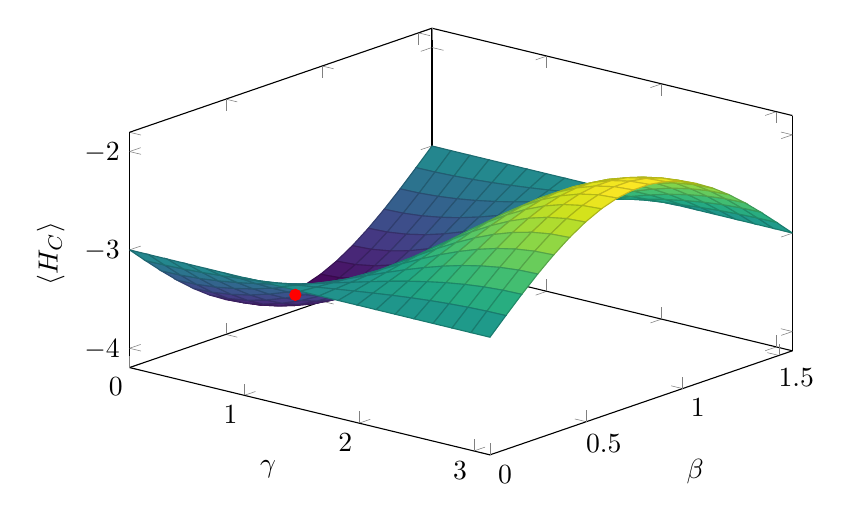
\begin{tikzpicture}
      \begin{axis}[
        width=10cm,
        height=7cm,
        xlabel=$\gamma$,
        ylabel=$\beta$,
        zlabel={$\langle H_C \rangle$},
        view={40}{30},
        colormap/viridis,
        ]

        \addplot3[
          surf,
          samples=20,
          domain=0:3.14,
          y domain=0:1.57,
          ]
          {-3 - cos(deg(x))*sin(deg(2*y))};

      % Optimal point
        \addplot3[only marks, mark=*, color=red] coordinates {(0.785, 0.393, -3.5)};
      \end{axis}
    \end{tikzpicture}
    \caption{Example landscape for \textsc{Max-Cut} QAOA with $P=1$ on a
    4-node cycle graph. The red dot indicates the optimal parameters.}
    \label{fig:landscape}
  \end{figure}
}

\vspace{0.3cm}

\index{Quantum Approximate Optimization Algorithms!Theoretical Insights}
\subsubsection*{Theoretical Insights for QAOA}

\noindent
\textbf{Adiabatic Quantum Computing Connection:}
\begin{itemize}
  \item As $P \to \infty$, QAOA approximates adiabatic quantum computing

  \item QAOA with optimal parameters can outperform the standard adiabatic
    algorithm

  \item For $P = poly(n)$, QAOA can capture quantum advantage for certain
    problems
\end{itemize}

\nt{
  The connection to adiabatic quantum computing suggests that QAOA can
  potentially solve NP-hard problems efficiently for specific instances,
  though this is not guaranteed in general.
}

\vspace{0.3cm}

\noindent
\textbf{Concentration of Parameters:}
\begin{itemize}
  \item For certain problems, optimal QAOA parameters concentrate (become
    instance-independent) as problem size grows

  \item This allows precomputing parameters for problem classes rather than
    instances

  \item Particularly relevant for local cost functions like \textsc{Max-Cut}
    on regular graphs
\end{itemize}

\ex{Parameter Concentration Example}{
  For \textsc{Max-Cut} on 3-regular graphs, optimal $\gamma$ and $\beta$
  values for $P=1$ are nearly identical across different random instances as
  the number of vertices increases. This means we can reuse the same
  parameters for any 3-regular graph without instance-specific optimization.
}

\begin{figure}[H]
  \centering
  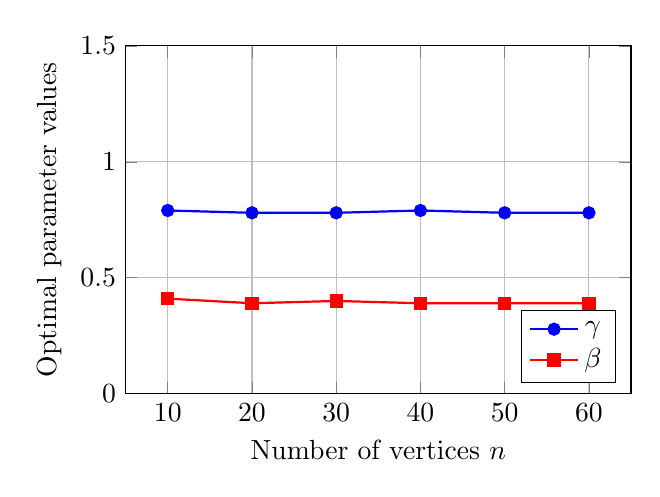
\begin{tikzpicture}
    \begin{axis}[
      width=8cm,
      height=6cm,
      xlabel={Number of vertices $n$},
      ylabel={Optimal parameter values},
      legend pos=south east,
      ymin=0, ymax=1.5,
      xtick={10, 20, 30, 40, 50, 60},
      grid=major
      ]

      \addplot[blue, mark=*, thick] coordinates {
        (10, 0.79)
        (20, 0.78)
        (30, 0.78)
        (40, 0.79)
        (50, 0.78)
        (60, 0.78)
      };

      \addplot[red, mark=square*, thick] coordinates {
        (10, 0.41)
        (20, 0.39)
        (30, 0.40)
        (40, 0.39)
        (50, 0.39)
        (60, 0.39)
      };

      \legend{$\gamma$, $\beta$}
    \end{axis}
  \end{tikzpicture}
  \caption{Parameter concentration for \textsc{Max-Cut} QAOA on 3-regular
  graphs}
  \label{fig:parameter-concentration}
\end{figure}


%%%%%%%%%%%%%%%%%%%%%%%%%%%%%%%%%%%%%%%%%%%%%%
% End of Lecture 14
%%%%%%%%%%%%%%%%%%%%%%%%%%%%%%%%%%%%%%%%%%%%%%
